\chapter{Equation of motion for angular motion}

Date: 29/10/2020

\section{Aim}
The aim of this experiment is to determine the angular acceleration and angular displacement for rotational motion using curve fitting in MATLAB. We also aim to derive equations of motion for rotational motion.


\section{Background Theory}

Rotational motion has similar characteristics to linear motion that is known as transnational motion. Rotational bodies have a moment of inertia similar to mass. The kinematics of rotational motion describes the relationships among rotation angle, angular velocity, angular displacement, angular acceleration, and time. Similar to linear motion equations, rotational motion equations can be written from the table provided in the manual. 
For linear equation $$ v=v_0 +at$$ Rotational can be written as following. In rotational $a = \alpha$ and $ a= r \alpha$ as angular acceleration is constant. $v=r \omega$ for rotational. Therefore 
$$ r \omega = r \omega_0 + r\alpha t $$ 
$$ \omega=\omega_0 + \alpha t$$
For linear equation $$ S= S_0 + v_i t + \frac{1}{2} a t^2$$. In rotational motion $S=\theta$ , $v=\omega$ , $a=\alpha$. Therefore 
$$\theta = \theta_0 + \omega_i t + \frac{1}{2} \alpha t^2 $$

% This section is meant to explain the theoretical background of the experiment whose report you are writing. Theoretical background \ref{eq:line} does not mean historical background. Be precise to, ONLY include scientific background.
% Table generated by Excel2LaTeX from sheet 'Sheet1'



% \begin{equation}
%     y = mx + c 
%     \label{eq:line}
% \end{equation}

% \begin{equation} \label{eq1}
% \begin{split}
% A & = \frac{\pi r^2}{2} \\
%  & = \frac{1}{2} \pi r^2
% \end{split}
% \end{equation}

\section{Description of Setup}
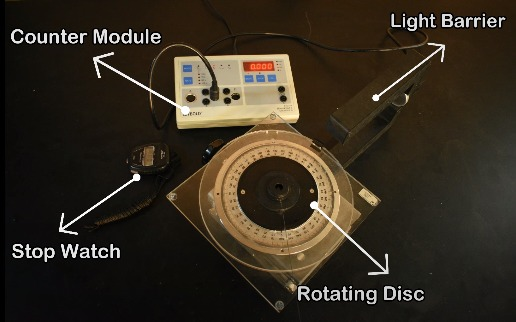
\includegraphics[width=10cm, height=7cm]{figures/exp6fig.jpeg} \\
Using the setup above, a light barrier is attached to the lab bench using a table clamp to place a rotating disk. The counter module and light barrier record the time when the flag interrupts the barrier. The stopwatch is used to record the time from rotation to when the main platter is detected. A pulley and thread help rotate the disk at constant acceleration. 
% Sketch and explain the experimental setup. The explanation should try to cover these pointers:  table \ref{tab:addlabel}
% \begin{enumerate}
%     \item What is the purpose of individual items in the setup?
%     \item If any equipment is taking measurements, what is it reading and how is it being read?
% \end{enumerate}

% Be precise to, ONLY include scientific description.

\section{Method / Procedure}

The experiment was set up and the disk was rotated at an angle of 90' and stopwatch was started when disk was released. The stop watch was stopped when the flag was detected by motion detector. 
The time measured by stopwatch and light gate at that angle was noted and repeated four times. 
The process was repeated five times by rotating disk at an angle of 120, 150, 180, 210, 240, 270 and 300'.
The respected data was recorded. 


% Highlight the following aspects of the experiment conducted 
% \begin{enumerate}
%     \item What method did you use to perform the experiment?
%     \item What adjustments were made, if any? 
%     \item What data was collected?
%     \item How was it collected?
%     \item Were any calibrations made and what were they?
% \end{enumerate}

% Be precise to, ONLY include scientific background.

\section{Data}

The type B uncertainty associated with the angle $\theta$ is 0.04 degrees. The type B associated uncertainty with the time T is $0.003$s

\begin{center}
\begin{tabular}{|l|l|l|}
\hline
\textbf{s.No} & \textbf{Angle} & \textbf{angle (°)} \\ \hline
1             & A1             & 90                 \\ \hline
2             & A2             & 120                \\ \hline
3             & A3             & 150                \\ \hline
4             & A4             & 180                \\ \hline
5             & A5             & 210                \\ \hline
6             & A6             & 240                \\ \hline
7             & A7             & 270                \\ \hline
8             & A8             & 300                \\ \hline
\end{tabular}
\end{center}

\begin{center}
  

\begin{tabular}{|l|l|l|l|l|l|l|l|l|}
\hline
\multicolumn{9}{|c|}{\textbf{Time period from Start to Cut}} \\ \hline
\textbf{s.No} &
  \textbf{T\_A1 (s)} &
  \textbf{T\_A2 (s)} &
  \textbf{T\_A3 (s)} &
  \textbf{T\_A4 (s)} &
  \textbf{T\_A5 (s)} &
  \textbf{T\_A6 (s)} &
  \textbf{T\_A7 (s)} &
  \textbf{T\_A8 (s)} \\ \hline
1  & 1.94  & 2.31  & 2.59 & 2.66 & 2.88 & 3.25 & 3.35 & 3.47 \\ \hline
2  & 1.93  & 2.31  & 2.65 & 3    & 3.03 & 2.84 & 3.35 & 3.35 \\ \hline
3  & 1.81  & 2.41  & 2.75 & 2.62 & 2.9  & 2.65 & 3.22 & 3.46 \\ \hline
4  & 2.03  & 2.34  & 2.84 & 2.69 & 2.75 & 3.19 & 3.34 & 3.42 \\ \hline
5  & 2.09  & 2.63  & 2.63 & 2.59 & 2.87 & 3.04 & 3.28 & 3.41 \\ \hline
\end{tabular}
\end{center}

\begin{center}
\begin{tabular}{|l|l|l|l|l|l|l|l|l|}
\hline
\multicolumn{9}{|c|}{\textbf{Time period from Start to Cut}} \\ \hline
\textbf{s.No} &
  \textbf{T\_A1 (s)} &
  \textbf{T\_A2 (s)} &
  \textbf{T\_A3 (s)} &
  \textbf{T\_A4 (s)} &
  \textbf{T\_A5 (s)} &
  \textbf{T\_A6 (s)} &
  \textbf{T\_A7 (s)} &
  \textbf{T\_A8 (s)} \\ \hline
1  & 1.94  & 2.31  & 2.59 & 2.66 & 2.88 & 3.25 & 3.35 & 3.47 \\ \hline
2  & 1.93  & 2.31  & 2.65 & 3    & 3.03 & 2.84 & 3.35 & 3.35 \\ \hline
3  & 1.81  & 2.41  & 2.75 & 2.62 & 2.9  & 2.65 & 3.22 & 3.46 \\ \hline
4  & 2.03  & 2.34  & 2.84 & 2.69 & 2.75 & 3.19 & 3.34 & 3.42 \\ \hline
5  & 2.09  & 2.63  & 2.63 & 2.59 & 2.87 & 3.04 & 3.28 & 3.41 \\ \hline
\end{tabular}
\end{center}

\begin{center}
\begin{tabular}{|l|l|l|}
\hline
Angle(rad) & Light Flag(s) & Stopwatch(s) \\ \hline
1.5707963  & 0.100081      & 1.96         \\ \hline
2.0943951  & 0.087436      & 2.4          \\ \hline
2.6179939  & 0.078868      & 2.692        \\ \hline
3.1415927  & 0.072822      & 2.712        \\ \hline
3.6651914  & 0.067409      & 2.886        \\ \hline
4.1887902  & 0.060538      & 2.994        \\ \hline
4.712389   & 0.060429      & 3.307        \\ \hline
5.2359878  & 0.056155      & 3.42167      \\ \hline
\end{tabular}
\end{center}

\newpage
\begin{figure}[h!]
    \centering
    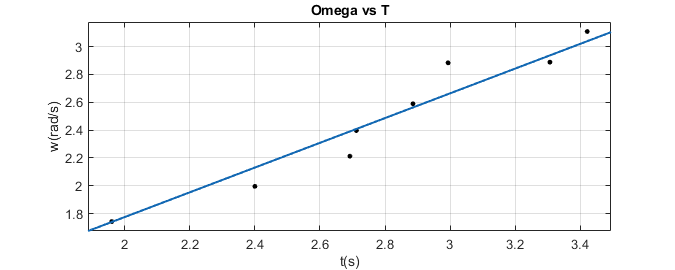
\includegraphics[width=\textwidth]{figures/omega_vs_t.png}
    \caption{Graph of $\omega$ vs t}
    \label{fig:yx}
\end{figure}
$$ \omega_f = \alpha t$$
$$ \alpha = 0.888 rad/s^2 $$


\begin{figure}[h!]
    \centering
    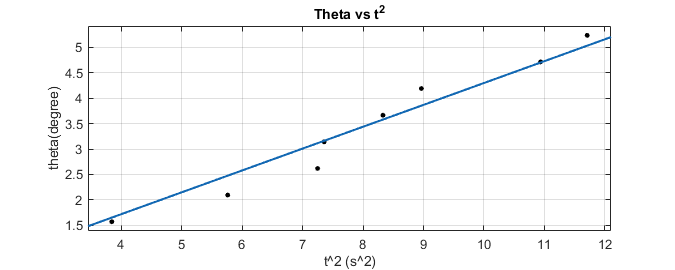
\includegraphics[width=\textwidth]{figures/theta_vs_t2.png}
    \caption{Graph of $\theta$ vs $t^2$}
    \label{fig:yx}
\end{figure}
$$ \theta = \alpha t^2$$
$$ \alpha = 0.430 rad/s^2 $$


\section{Data Analysis}

\newpage
\begin{figure}[h!]
    \centering
    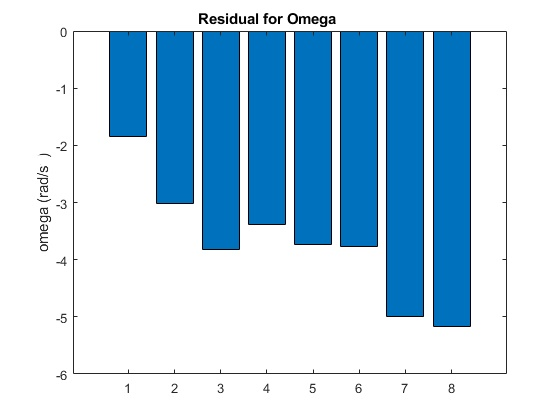
\includegraphics[width=\textwidth]{figures/res_omega.jpg}
    \caption{Residual plot for omega}
    \label{fig:yx}
\end{figure}


\newpage
\begin{figure}[h!]
    \centering
    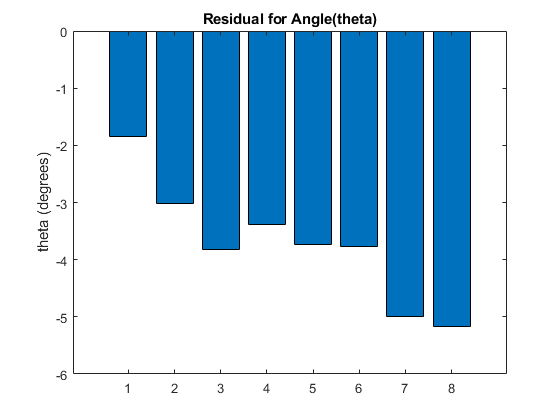
\includegraphics[width=\textwidth]{figures/res_theta.png}
    \caption{Residual plot for theta}
    \label{fig:yx}
\end{figure}


\section{Discussion \& Conclusion}

The graphs of $\omega$ vs t and $\theta$ vs $t^2$ are linear with an equal distribution of points on line as predicted by our hypothesis which verifies the equations of angular motion. There is a degree of uncertainty and error in the instruments while measuring time and angle, 0.04 for angle and 0.003 for time respectively. Reasons for points varying from the exact position on line include human error while measuring the time from stopwatch. Friction in the pulley, air resistance can also affect our experimental values. The degree of errors is increasing with increasing omega as seen in figure 6.3. 

% Summarize and discuss the experimental results, what do the results say about your hypothesis, if such a hypothesis was made for the experiment. Mention the uncertainty in the calculated quantity Be precise and only include scientific discussion.


\section{MATLAB Script}
\lstinputlisting{matlabCodes/Experiment6.m}



